\subsection{Разработка технического задания}
\subsubsection{Постановка задачи проектирования}

Целью разработки подсистемы автономного определения перемещения объекта является предоставления удобного с точки зрения интеграции компонента для встраивания во многие бытовые автономные автоматические системы,  в то же время дешевого и не требующего специализированных устройств для своей работы.

\subsubsection{Описание предметной области}
\paragraph{Естественно-языковое описание процесса.}

В ходе создания подвижных автономных систем возникает задача определения текущего местоположения объекта в пространстве.

Для этого можно использовать различные методы, основанные на глобальном позиционировании в географической системе координат с использованием позиционирования по спутникам (GPS, ГЛОНАСС), или методы, основанные на определении перемещения от стартовой позиции. При этом у данных методов разные сферы применения. Так, например, при позиционировании внутри помещения использование спутниковых систем позиционирвоания становиться невозможным по причине слабого сигнала или его полного отсутсвтвия, а так же из-за недостаточной точности в рамках навигации внутри интерьера помещения. Так же не стоит забывать про акутальность систем навигации в космической отрасли, где использование спутников является невозможным впринципе. 
Вторую группу методов принято называть методами одометрии, которые могут быть основаны на:
\begin{itemize}
\item на вращении колес;
\item использовании инерциальных измерительных приборов;
\item компьютерном зрении.
\end{itemize}

Каждый из них обладает своими плюсами и минусами \cite{odometryMethods}, но развитие вычислительной техники и алгоритмов компьютерного зрения дало мощный толчок к более широкому применению визуальной одометрии. Данный подход позволяет получать один видеоряд через видеокамеру и на его основе получать разные сведения об окружающей среде. Тем не менее он не лишен недостатков. Для борьбы с ними применяется комбинация нескольких методов одомтерии. 

Одним из вариантов сомещения методов является использование метода визуальной одометрии и инерционных измерительных устройств. 

При таком гибридном методе данные с видеокамеры и данные с инерционных измерительных устройств обрабатываются параллельно и независимо. В результате получаются два независимых рассчитынных положения носителя, после чего они сопоставляются, и из них выбираются наиболее правдоподобные. 

Таким образом, в процессе функционирования спроектированного модуля визуальной одометрии происходит следующий бесконечный процесс. 
На вход модуля непрерывно подается видео поток и данные об угловых скоростях и ускорении объекта относительно трех взаимноперпендикулярных осей. Эти данные обрабатываются параллельно в соответствующих модулях, на выходе каждого из которых получаем смещение объекта относительно предыдущего положения и его поворот. Далее эти данные совмещаются и выбираются наиболее правдоподобные, которые затем прибавляются к положению и углу поворота, высчитанным на предыдущей итерации. 


\paragraph{Графическое представление процесса}
Графическое представление процесса процесса представлено на рисунке~\ref{pic:predmetOblast}.

\begin{figure}[!htb]
\center{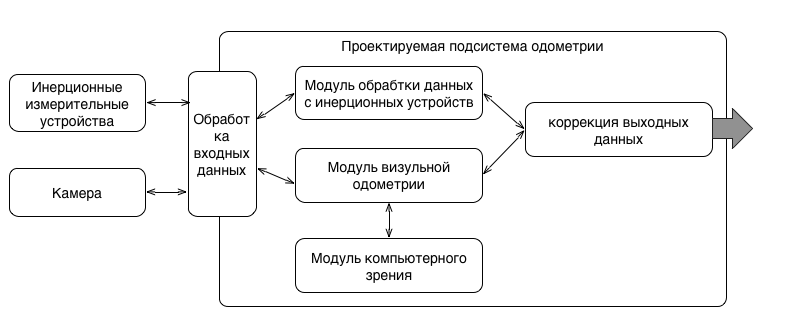
\includegraphics[width=0.8\linewidth]{pics/predmetOblast.png}}
\caption{Графическое представление процесса.}
\label{pic:predmetOblast}
\end{figure}

\paragraph{Вычисление оптического потока.}

\textbf{Оптический поток} — это изображение видимого движения объектов, поверхностей или краев сцены, получаемое в результате перемещения наблюдателя (глаз или камеры) относительно сцены\cite{wikiOpticalFlow}.

Существует несколько подходов к определению смещений между двумя соседними кадрами. Например, можно для каждого небольшого фрагмента (скажем, 8 на 8 пикселей) одного кадра найти наиболее похожий фрагмент на следующем кадре. В этом случае разность координат исходного и найденного фрагментов даст нам смещение. Основная сложность тут состоит в том, как быстро отыскать нужный фрагмент, не перебирая весь кадр пиксель за пикселем. Различные реализации этого подхода так или иначе решают проблему вычислительной сложности. Некоторые настолько успешно, что применяются, например, в распространенных стандартах сжатия видео. Платой за скорость естественно является качество. Мы же рассмотрим другой подход, который позволяет получить смещения не для фрагментов, а для каждого отдельного пикселя, и применяется тогда, когда скорость не столь критична. Именно с ним в литературе часто связывают термин “оптический поток”.

Данный подход часто называют дифференциальным, поскольку в его основе лежит вычисление частных производных по горизонтальному и вертикальному направлениям изображения. Как мы увидим далее, одних только производных недостаточно чтобы определить смещения. Именно поэтому на базе одной простой идеи появилось великое множество методов, каждый из которых использует какую-нибудь свою математическую пляску с бубном, чтобы достичь цели. Сконцентрируемся на методе Лукаса-Канаде (Lucas-Kanade), предложенном в 81 году Брюсом Лукасом и Такео Канаде. Данный метод является наименее ресурсоемким  \cite{habrOpticalFlowAbout} при этом обеспечивает приемлемое качество вычисления оптического потока. 

С математической точки зрения данный алгоритм можно описать следующим образом.
Пусть даны два изображения $F1$ и $F2$, и нам требуется найти смещение точки с координотой $x$. Рассматривая два последовательных изображения можно сказать:
$$ f_2(x) = f_1 (x-d)$$
Обратите внимание, что $f_1$ и $f_2$ при желании можно записать и в общем виде: $f_1(x) = I (x, y, t)$ ; $f_2(x) = I (x, y, t+1)$.

Свяжем известные значения со смещением d. Для этого запишем разложение в ряд Тейлора для $ f_1 (x-d)$:
$$  f_1 (x-d) =f_1(x) + df_1'(x) + O(d^2f_1'') $$
Предположим, что $ f_1 (x-d)$ достаточно хорошо аппроксимируется первой производной. Сделав это предположение, отбросим всё что после первой производной:
$$  f_1 (x-d) =f_1(x) + df_1'(x) $$

Смещение $d$ — это наша искомая величина, поэтому необходимо преобразовать $ f_1 (x-d)$ . Как мы условились ранее, $ f_2(x) = f_1 (x-d) $, поэтому просто перепишем:
$$ f_2(x)= f_1(x) - df_1'(x) $$
Отсюда следует:
$$ d = \frac{f_1(x)-f_2(x)}{f_1'(x)} $$

Следует отметить, что выше был рассмотрен одномерный случай и были сделаны несколько грубых допущений. Но описание алгоритма Лукаса-Канаде для двумерного случая только усложняет математические выводы и понимание сути. 

Для снижения погрешности вызванной отбрасыванием старших производных смещение для каждой пары кадров (назовём их $F_i$ и $F_{i+1}$) можно вычислять итеративно. В литературе это называется искажением (warping). На практике это означает, что, вычислив смещения на первой итерации, мы перемещаем каждый пиксель кадра $F_{i+1}$ в противоположную сторону так, чтобы это смещение компенсировать. На следующей итерации вместо исходного кадра $F_{i+1}$ мы будем использовать его искаженный вариант $F_{i+1}^1$. И так далее, пока на очередной итерации все полученные смещения не окажутся меньше заданного порогового значения. Итоговое смещение для каждого конкретного пикселя мы получаем как сумму его смещений на всех итерациях \cite{habrOpticalFlowTheory}.

Так же следует отметить, что данный алгоритм плохо работает на однотонных изображениях. Данный недостаток является самым критичным. 

\paragraph{Одометрия с использованием инерциальных измерительных устройств}
Навигационные решения надлежащего качества могут быть получены именно в результате взаимодействия или последующей совместной обработки данных от двух  источников - визуальной одометрии и инерциальной системы.  

В наиболее общей форме можно определить инерциальную систему как ортогональную триаду гироскопов и акселерометров, выполняющих непосредственные геопространственные измерения и вычислительный блок, осуществляющий алгоритмические преобразования данных непосредственных измерений.

Следует отметить, что гироскоп любого типа позволяет определять ориентацию в геодезическом пространстве в любой момент времени независимости от местоположения, скорости и других параметров носителя. Точность поставляемых гироскопом данных во всех случаях подвержена деградации («ухода») с течением времени. Величина «ухода» значительна и может составлять до нескольких градусов в час \cite{laserLocation}.

Акселерометры предназначены для измерения линейных ускорений. В равной степени они пригодны для измерений сил, так как согласно ньютоновской механике сила и ускорение есть разные проявления одного и того же физического явления.

В общем случае в системах навигации следует определять следующие показатели:
\begin{itemize}
\item \textbf{Рыскание} — угловые движения летательного аппарата, судна, автомобиля относительно вертикальной оси (см. также вертикальная ось самолёта), а также небольшие изменения курса вправо или влево, свойственные судну \cite{wikiRiskanie};
\item \textbf{Крен} — поворот объекта (судна, самолёта, фундамента) вокруг его продольной оси \cite{wikiKren};
\item \textbf{Тангаж} — угловое движение летательного аппарата или судна относительно главной (горизонтальной) поперечной оси инерции \cite{wikiTangazh}.

\end{itemize}
С учетом сделанных замечаний рассмотрим основные процедуры, выполняемые в навигационном комплексе на базисном уровне.

\textit{\textbf{Вычисление крена и тангажа посредством акселерометров}}

Обладая чувствительностью к земной гравитации, акселерометры обеспечивают измерение долговременных значений крена и тангажа по схеме, изображенной на рисунке~\ref{pic:tangazh}. Рассмотрим акселерометр, рабочая ось которого совпадает со строительной осью $oX$ носителя.

\begin{figure}[!htb]
\center{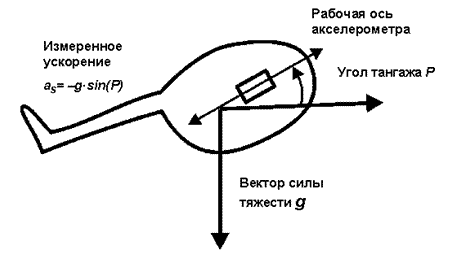
\includegraphics[width=0.6\linewidth]{pics/tangazh.png}}
\caption{Измерения величин крена и тангажа посредством акселерометров.}
\label{pic:tangazh}
\end{figure}

Полагая ускорение носителя равным нулю, мы можем вычислить угол тангажа как:
$$P = \arcsin (-a_s/g)$$

Аналогично вычисляется угол крена. Таким образом, два из трех углов, определяющих угловую ориентацию, могут быть определены только за счет использования акселерометров. Это совершенно очевидный результат, принимая во внимание то обстоятельство, что углы крена и тангажа по изначально определены по отношению к вертикали, которая в нашем случае соответствует вектору тяжести. Однако, здесь следует признать, что описанный метод не может быть использован на практике сам по себе, так как в описанной схеме существенно состояние покоя, в котором должна находиться система. Если это условие не соблюдается, то совершенно очевидно, что отсутствует принципиальная возможность выделить вектор ускорения свободного падения из суммы всех ускорений, которую испытывает система.

\textit{\textbf{Вычисление изменений ориентации с использованием гироскопов}}

Как отмечено выше, в конструкции навигационного комплекса используются оптические гироскопы, обладающие чувствительностью к изменениям ориентации т.е. к величине угловой скорости. Интегрирование (численное суммирование) значений, измеренных гироскопами, обеспечивает определение кратковременных угловых перемещений в физическом пространстве.

Для корректного расчета угла поворота должны быть учтены
внутренние ошибки гироскопа – дрейф, ошибка масштабного коэффициента, случайный шум.

\label{ref:dreif0}
При этом внутренние ошибки  гироскопа полностью смешаны с истинными значениями и не могут быть отделены от них на базисном информационном уровне. В процессе дальнейшей обработки эта смесь подвергается интегрированию, в результате чего возникает ошибочное угловое смещение, которое, таким образом, приобретает долговременный характер (рис. ~\ref{pic:acell}). Точная оценка величины ошибочного углового смещения и его устранение осуществляется при генерации навигационного решения на последующем навигационном уровне.

\begin{figure}[!htb]
\center{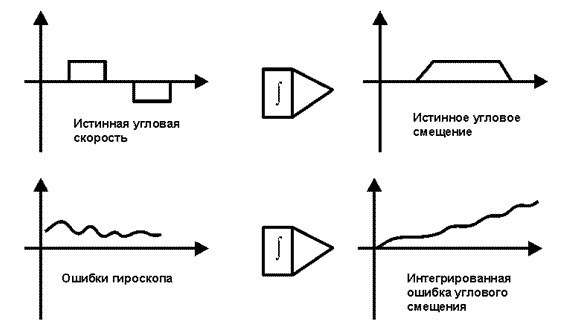
\includegraphics[width=0.6\linewidth]{pics/acelerometr.png}}
\caption{Схема определения углового смещения.}
\label{pic:acell}
\end{figure}

\textit{\textbf{Определение координат пространственного положения с помощью акселерометров.}}

Наличие акселерометров позволяет определять величины линейных ускорений, которые испытывает система. Положим, что ориентация системы в физическом пространстве определена точно с помощью методов, описанных выше. Тогда имеется возможность выделить вектор силы гравитации среди всей суммы векторов сил, приложенных к системе и, следовательно, оценить величину ускорения. Численное интегрирование ускорения позволяет перейти к скорости, а повторное интегрирование к перемещению. Таким образом, с учетом представленных выше замечаний и правилах перехода из физического пространства в географическое, появляется принципиальная возможность оценить геодезические координаты системы в любой момент времени.

\paragraph{Корректировка выходных данных}
\label{item:outputCorrect}
Так как процессы определения координат с использованием инерциальных устройсвт и визуальной одометрии проходят паралелльно, то на выходе получаются два значения для $x$, для $y$ и для $\alpha$.  

Практика показывает, что значения полученые при использовании визуальной одометрии более точные и величина ошибки меньше зависит от времени, в то время как инерциальные приборы подвержены <<дрейфу нуля>>, о чем сказано в пункте \ref{ref:dreif0}.

Однако при передвижении по однотонной поверхности, на которой алгоритм выделения ключевых точек дает сбой, визульная одометрия может давать совершенно нерпедсказуемые результаты. На практике это выражается в резком изменении выходных значений $x$, $y$, $\alpha$. 

В связи с этим, данные, полученые с использованием инерциальных устройсвт и визуальной одометрии, следует проверять на правдивость. 

Следует выделить следующие контрольные величины, изменение которые следует учитывать.
\begin{enumerate}
\item Скорость пермещения. 

Чаще всего известна максимальная скорость передвижения камеры, ограниченная максимальной скоростью перемещения ее носителя. Важно понимать, что $x$, $y$ и $\alpha$ это изменения соотвествующих параметров положения носителя в пространстве. Для перехода от них к скорости можно воспользоваться следующей формулой:
 $$ V \cdot \bigtriangleup t = x^2 + y^2 $$

При обработке видеофайла можно узнать частоту кадров, которая чаще всего составляет 22 или 30 кадров в секунду. Тогда временной интервал между двумя кадрами, а следовально и между двумя итерациями работы алгоритма визуальной одометрии составляет $1/22 \approx 45 мс$ и $ 1/30 \approx 33 мс$ соответственно. Будем обозначать этот интеревал времени через $\bigtriangleup t$.

Таким образом можно установить следущий сигнальный показатель ошибки в работе алгоритма визульной одометрии:
$$  x^2 + y^2  \leqslant V_{макс} \cdot \bigtriangleup t = 
\frac{x^2 + y^2}{\bigtriangleup t} \leqslant V_{макс}
$$

\item Абсолютная скорость изменения параметров.

Так как измеритльные устройства расположены на каком-либо физическом носителе, и этот носитель обладает некоторой инерционностью, то скрость изменения параметров не должна быть выше, чем это позволяют динамические параметры носителя. Скорость изменения параметров есть ни что иное, как первая производная. Но если учитывать, что  $x$, $y$ и $\alpha$ это изменения соотвествующих параметров положения носителя в пространстве, то необходимо ограничивать их величину на единицу времени. 



Введем следующие сигнальные показатели:
\begin{itemize}
\item $x/ \bigtriangleup t \leqslant V_{макс}^x = V_{макс}$
\item $y / \bigtriangleup t \leqslant V_{макс}^y = V_{макс}$
\item $\alpha / \bigtriangleup t \leqslant V_{макс}^{\alpha}$
\end{itemize}

\item Относительная скорость изменения параметров.

Так же как и в предыдущем пункте, инерционность носителя устройств накладывет ограничения на изменения парамтеров относительно предыдущей итерации. 
Пусть $x_{пред}$ - значение, полученное не предыдущей итерации алгоритма визуальной одометрии, а  $x_{тек}$ - текущее значение. 
Таким образом $ x_{тек} - x_{пред}$ - разница в изменении положения носителя за два временных отрезка. 
С учетом физических ограничений, получаем:
$$ x_{тек} - x_{пред} \leq \bigtriangleup X_{max}$$

Аналогично получаем для $y$ и $\alpha$:
$$ y_{тек} - y_{пред} \leq \bigtriangleup Y_{max}$$
$$ \alpha_{тек} - \alpha_{пред} \leq \bigtriangleup \alpha_{max}$$

Для угла поворота следует учитывать то, что этот показатель может колебаться в пределах от $0^\circ$ до $360^\circ$, и значение $\alpha$ следует брать исключительно до аккумулирования с общими значениями.  
\end{enumerate}


\paragraph{Анализ функций, подлежащих автоматизации}
Исходя из сказанного выше, можно выделелить следующие функции, подлежащие автоматизации.
\begin{itemize}
\item Вычисление оптического потока.
\item Обработка инерциальных данных и вычисление смещения
\item Сопоставление полученных данных и выбор наилучшего результата. 
\end{itemize}

\subsubsection{Выбор критериев качества}
Выделим основные критерии, по которым следует оценивать разрабатываемую подсистему.
\begin{itemize}
\item \textbf{Необходимость в специальном оборудовании} - исходя из задачи, предполагается использование проектируемого модуля в низкобюджетных системах. В связи с этим необходимо обеспечить корректную работу подсистемы с неспециальным оборудованием таким, как бытовые камеры. 
\item \textbf{Стоимость необходимого оборудования} – исходя из предыдущего пункта, следует обеспечивать поддержку наиболее дешевого оборудования. 
\item \textbf{Сложность интеграции} – в современном мире наличия многих конкурентов и налогов одним из ключевых факторов при выборе между ними является простота использования продукта. В связи с этим необходимо снизить время, необходимое на интеграцию с разрабатываемой подсистемой, путем предоставления удобного в использовании API.
\item \textbf{Точность} - данный критерия является важным для задач определения положения в пространстве априори, так как при низкой точности использование систем данного рода становится бесмысленным. Тем не менее в рамках многих задач обеспечение чрезмерно высокой точности является избыточным.
\item \textbf{Возможность свободного использования} – нередко разработчики программных или аппаратных продуктов накладыают ограничение в виде разного рода лицензий распространения, которые ограничивают пользователей в распространении и использовании своих продуктов. В связи с этим важным явлется свободность использования продукта в любых целях, не  противоречящих законодательству стран, где проихсходит его использование.
\end{itemize}

\subsubsection{Анализ аналогов и прототипов}

\paragraph{ROS Odometry}
ROS (Robot Operating System) — Операционная система для роботов — это фреймворк для программирования роботов, предоставляющий функциональность для распределённой работы. ROS был первоначально разработан в 2007 году под названием switchyard в Лаборатории Искусственного Интеллекта Стэнфордского Университета для проекта (STAIR). В 2008 году развитие продолжается в Willow Garage, научно-исследовательском институте/инкубаторе робототехники, совместно с более чем двадцатью сотрудничающими институтами.

ROS обеспечивает стандартные службы операционной системы, такие как: аппаратную абстракцию, низкоуровневый контроль устройств, реализацию часто используемых функций, передачу сообщений между процессами, и управление пакетами. ROS основан на архитектуре графов, где обработка данных происходит в узлах, которые могут получать и передавать сообщения между собой. Библиотека ориентирована на Unix-подобные системы (Ubuntu Linux включен в список «поддерживаемых» в то время как другие варианты, такие как Fedora и Mac OS X считаются «экспериментальными»).

ROS имеет две основные «стороны»: стороны операционной системы ros, как описано выше и ros-pkg, набор поддерживаемых пользователями пакетов (организованных в наборы, которые называются стек), которые реализуют различные функции робототехники: SLAM, планирование, восприятие, моделирование и др.\cite{wikiROS}

В состав ROS так же входят различные пакеты одометрии, наиболее приемлемым является пакет LIBVISO2 \cite{libvis1}.

LIBVISO2 (библиотека для визуальной одометрии, версия 2) является очень быстрой кроссплатформенной библиотекой, написанной на C++ с MATLAB оберткой для использования. Основная цель библиотеки – вычисление 6 DOF движения движущеся моно/стерео камеры. Не будем подробно рассматривать стереоверсию библиотеки, так как этот класс одометрии лежит в другой плоскости. Монокулярная версия на данный момент ещенаходится в статусе экспериментальной и использует 8-ми точечный алгоритм для фундаментальной оценки матрицы. Кроме того, он предполагает, что камера движется при известной и фиксированной высоте над землей (для оценки масштаба). 

Чтобы оценить масштаб движения, моноодометр использует горизонтальную плоскость и, следовательно, нуждается в информации о z-координате и углу наклона камеры.

В общем случае, монокулярная одометрия и SLAM-системы не могут оценить движение или положение на метрической шкале. Libviso2 разрешает эту неопределенность через фиксированный переход от плоскости земли к камере. Для этого и необходимо знать параметры camera height и camera pitch (высота камеры и ее угол наклона). Эти значения должны быть оценены и введены в систему вручную при каждой установке камеры на объект\cite{libvis2}. 

Кроме того, существует еще одна проблема: когда камера выполняет только чистое вращение, матрицы для решения СЛАУ вырождаются, и, даже если система очень мощная, алгоритм пересает корректно работать.


\paragraph{Project Tango}
Небольшая группа инженеров ATAP (Advanced Technology and Projects) в компании Google занимается разработкой перспективных технологий. Сегодня она представила свой новый проект Tango. Это очень красивая технология построения 3D-модели окружающего пространства с помощью смартфона.

Группа ATAP сконструировала 5-дюймовый смартфон, оснащённый стереокамерой, сенсорами и программным обеспечением, которые отслеживают положение смартфона в 3D-пространстве, а также сканируют окружающий мир в реальном времени со скоростью 250 тыс. измерений в секунду. Всё это объединяется в единую 3D-модель с помощью уникального процессора Myriad 1, разработанного стартапом Movidius.

Когда модель готова, телефон может постоянно определять своё местоположение внутри неё. На базе этой модели можно создавать интересные игры, когда виртуальные объекты в смартфоне совмещаются с реальными объектами окружающей действительности. Например, вы можете играть на смартфоне в футбол, отбивая мячик от стены собственной квартиры. Или управлять настоящим роботом в соседней комнате, двигая его по 3D-модели этой комнаты. Или играть в прятки с анимированным персонажем в своём собственном доме. В общем, возможности открываются невероятные.

В ближайшие месяцы ATAP намерены выпустить SDK для создания программ на новом оборудовании. Первые 200 устройств разошлют разработчикам после 14 марта. Чтобы принять участие в программе, нужно придумать интересное приложение в сфере навигации внутри помещений, игр для одного или нескольких игроков или алгоритмы обработки данных с сенсоров Tango.

Телефон работает под Android, так что API для доступа к информации об ориентации, позиционировании и расстоянии до объектов можно использовать со стандартными Android-приложениями, написанными на Java, C/C++, а также на игровом движке Unity. Первые версии алгоритмов и API скоро закончат, но проект и после этого останется в статусе эксперимента \cite{habrTango}\cite{googleTango}.

\paragraph{SMP Robotics}
Компания SMP Robotics занимается созданием беспилотных транспортных средств и в их роботах серии «SRX» реализован принцип визуального определения местоположения робота.

Назначение роботов этой серии — езда по известному маршруту, особенности которого хранятся в бортовом компьютере робота в виде карты со множеством характеристик условий путей проездов. Более того, робот, многократно проезжая по одним и тем же участкам, может уточнять и накапливать данные о них на протяжении дня и ночи, сезонных или погодных изменениях окружающего ландшафта.

Всё это позволило успешно применить алгоритм визуального определения местоположения робота на основе анализа и последующего сравнения видеоизображений, полученных при первичном и последующем проездах.
Первичный проезд можно рассматривать как обучающий, в нём формируется набор ключевых кадров, которые позволяют сформировать базу данных, описывающую взаиморасположение устойчивых структур. При последующем автоматическом движении характеристики текущего изображения проверяются на тождественность описаний, хранящихся в базе данных, и, при их совпадении, осуществляется привязка к текущему местоположению.

В условиях циклических проездов робота по одному и тому же маршруту появляется возможность автоматического пополнения и уточнения базы данных взаиморасположения устойчивых структур на видео с курсовой камеры. Накопленные данные будут коррелировать со сменой дня и ночи, сезонными изменениями ландшафта, особыми погодными условиями. Расширенная база данных позволяет произвести достоверное сопоставление большому количеству текущих кадров видеоизображения к ранее обработанным и сохранённым кадрам известной траектории движения, тем самым достигнуть точного определения местоположения на большинстве участков траектории движения и, соответственно, повысить скорость автоматического проезда по известному маршруту.

Используемый метод визуального определения местоположения и управления движением позволяет переносить накопленную информацию о маршруте движения от одного робота к другому. Робот, проехавший по маршруту много раз, сформирует достаточно полную базу данных о его характеристиках. База данных может быть установлена на новый робот, который еще ни разу не проходил по данному маршруту, и он успешно проедет по нему с достаточной точностью и предельно возможной скоростью.
Возможность копирования и обмена данными о маршруте, накопленными алгоритмом визуального определения местоположения, особенно полезна при проездах по значительным территориям. На начальном этапе несколько роботов накапливают информацию на локальных участках, при достижении её достаточного качества, все данные объединяются в единую базу данных и представляют собой информацию о маршруте в целом. Объём этих данных позволяет каждому из роботов проехать все участки маршрута, не смотря на то, что конкретно этот робот там никогда не ездил. Информация о маршруте длительное время остается достоверной. Несмотря на естественные изменения ландшафта, адаптивность алгоритма позволяет скорректировать массив данных даже при значительных изменениях окружающей обстановки, а при последующих проездах снова пополнить его новыми данными.

Метод визуального определения местоположения позволяет обойтись без внешних, по отношению к движущемуся роботу, компонентов системы. Информации, полученной в результате обработки изображения окружающего ландшафта, достаточно для достоверного принятия решения о выборе пути движения. И это — коренное отличие описываемого подхода по сравнению с известным методом высокоточного вождения по данным от дифференциального приемника спутниковой навигационной системы. Такая система требует не только прямой видимости на спутниковую группировку, но и базовой корректирующей станции в зоне радиовидимости робота. В реальных условиях эксплуатации каналы связи, как со спутниками, так и с базовой станцией нельзя считать надежным. Даже в городском лесопарке с низкой плотностью деревьев получить достоверные данные от спутниковой навигационной системы практически невозможно, кроме того, существуют зоны радио тени, обусловленные застройкой. Высокочастотный спутниковый сигнал подвержен серьезному ослаблению даже во время незначительных осадков, мокрая листва деревьев вносит достаточное ослабление, чтобы сделать спутниковую группировку радио невидимой. В целом, метод высокоточного вождения по данным от дифференциального приемника спутниковой навигационной системы, хорош в условиях, для которых он и разрабатывался — для автоматического вождения сельскохозяйственной техники в чистом поле и, желательно, без дождя.

Управление движением посредством анализа видеоизображений окружающей обстановки и визуального определения местоположения обеспечивает полную автономность движения наземного робота. И, в отличие от других рассмотренных методов, не требует ни внешней инфраструктуры, ни устойчивых каналов связи с дополнительным оборудованием \cite{spmrobotics}.


\paragraph{Сравнительный анализ}

Для сравнения представленных вариантов воспользуемся методом взвешенной суммы. Данный метод позволяет объединить ряд критериев сравнения в один интегральный показатель, по которому затем выбирается наилучший вариант, соответствующий максимальному значению этого интегрального показателя. Метод взвешенной суммы можно представить следующим образом: 
$$ Y = \max_{j \ni m} \displaystyle\sum_{i=1}^{n} \alpha_i \cdot K_{ij},$$
где $\sum_{i=1}^{n} \alpha_i = 1$

По этому критерию проводится сравнение $j (j = 1, 2, …, m)$ вариантов по $i (i = 1, 2, …, n)$ показателям, где:

$n$ – количество показателей сравнения;

$m$ – количество вариантов сравнения.

$K_{ij}$ – нормированный коэффициент соответствия $i$-ого параметра $j$-ого варианта эталонному значению, т.е. для $j$-ого варианта:
$$ K_{ij} = \frac{\max_{j} X_{ij}} {X_{ij}}, $$
$$ 0 < K_{ij} < 1 $$
Соответствие систем-аналогов выбранным критериям качества представлено в Таблице~\ref{tab:srav_ling}.

\begin{table}[!htb]
	\caption{Сравнение аналогов. Лингвистические оценки.}\label{tab:srav_ling}
    \centering
	\begin{tabular}{|p{4cm}|p{4cm}|p{2cm}|p{2cm}|p{2cm}|}
	\hline 
	\multirow{2}{4cm}{Критерий} & \multirow{2}{4cm}{Проектируемая подсистема} & 	\multicolumn{3}{c|}{Аналоги}\\ 
	\cline{3-5}
	 &   & ROS odometry & Project tango & SMP Robotics \\ 
	\hline 
	Необходимость в специальном оборудовании. & Нет & Нет & Да & Да \\ 
	\hline 
	Стоимость необходимого оборудования & Низкая & Средняя & Средняя & Высокая \\ 	
	\hline 
	Сложность интеграции. & Низкая & Высокая & Низкая & Средняя \\
	\hline 
	Точность. & Средняя & Высокая & Высокая & Высокая \\ 
	\hline 
	Возможность свободного использования. & Есть & Есть & Есть & Нет \\ 
	\hline 
	\end{tabular}
\end{table} 

Для сравнений необходимо перевести качественные оценки в количественные. Метод перевода для каждого из критериев представлен в таблицах ниже.

\begin{table}[!htb]
	\caption{Сравнение аналогов. Лингвистические оценки.}
    \centering
	\begin{tabular}{|p{3cm}|p{6cm}|p{6cm}|}
	\hline 
	Описание & Для функционирования системы необходимы специфические устройства, или устройства с повышенными точностями & Система может функционировать на любом оборудовании и это оборудовании не сложно найти \\ 
	\hline 
	Лингв. оценка & Да & Нет \\ 
	\hline 
	Балл & 0,4 & 1 \\ 
	\hline 
	\end{tabular} 
\end{table} 

\begin{table}[!htb]
	\caption{Перевод качественных оценок в количественные для критерия 
  <<Стоимость необходимого оборудования>>}
    \centering
	\begin{tabular}{|p{3cm}|p{4,5cm}|p{4,5cm}|p{4,5cm}|}
	\hline 
	Описание & 
	Стоимость необходимого оборудования исчисляется десятками тысяч рублей & 
	Стоимость оборудования лежи в диапазоне от 5 000 до 20 000 рублей &
	Стоимость оборудования составляет менее 5 000 рублей \\ 
	\hline 
	Лингв. оценка & Высокая & Средняя & Низкая \\ 
	\hline 
	Балл & 0,1 & 0,6 & 1 \\ 
	\hline 
	\end{tabular} 
\end{table} 

\begin{table}[!htb]
	\caption{Перевод качественных оценок в количественные для критерия 
  <<Сложность интеграции>>}
    \centering
	\begin{tabular}{|p{3cm}|p{4,5cm}|p{4,5cm}|p{4,5cm}|}
	\hline 
	Описание & 
	Данную систему сложно интегрировать с другими системами, потребуются серьезные доработки & 
	Данную систему можно интегрировать с другими системами, но для этого необходимы доработки обеих систем &
	Данную систему легко интегрировать с другими системами, стоимость и время доработок низкие \\ 
	\hline 
	Лингв. оценка & Высокая & Средняя & Низкая \\ 
	\hline 
	Балл & 0,1 & 0,6 & 1 \\ 
	\hline 
	\end{tabular} 
\end{table} 

\begin{table}[!htb]
	\caption{Перевод качественных оценок в количественные для критерия 
  <<Точность>>}
    \centering
	\begin{tabular}{|p{3cm}|p{4,5cm}|p{4,5cm}|p{4,5cm}|}
	\hline 
	Описание & 
	Точность ограничена лишь точностью используемого оборудования, со временем увеличение ошибки не наблюдается. & 
	Используемые алгоритмы допускают определенную погрешность, со временем возможно увеличение ошибки &
	Точность вычислений крайне низкая, со временем наблюдается накапливание ошибки \\ 
	\hline 
	Лингв. оценка & Высокая & Средняя & Низкая \\ 
	\hline 
	Балл & 1 & 0,6 & 0,1 \\ 
	\hline 
	\end{tabular} 
\end{table} 

\begin{table}[!htb]
	\caption{Перевод качественных оценок в количественные для критерия 
  <<Возможность свободного использования>>}
    \centering
	\begin{tabular}{|p{3cm}|p{6cm}|p{6cm}|}
	\hline 
	Описание & 
	Исходные коды открыты, допускается свободное использование & 
	Система является проприетарной \\ 
	\hline 
	Лингв. оценка & Да & Нет \\ 
	\hline 
	Балл & 1 & 0,4 \\ 
	\hline 
	\end{tabular} 
\end{table} 

Учтём весовой коэффициент. Для этого каждому критерию зададим весовой коэффициент, кратный х - минимальному весовому коэффициенту:
\begin{enumerate}
\item Необходимость в специальном оборудовании – $3х$
\item Стоимость необходимого оборудования – $3х$
\item Сложность интеграции – $2х$
\item Точность – $2х$
\item Возможность свободного использования – $1х$
\end{enumerate}

Сумма весовых коэффициентов по всем критериям качества равна 1.
$$3х + 3х + 2х + 2х + 1х = 11х => х = 0,0909$$
Таким образом, можно составить сравнительную таблицу, содержащую количественные и качественные оценки и подсчитать итог, метом взвешенной суммы.
Итоговое сравнение с учетом весового коэфициента и количественных оценок приведены в Таблице~\ref{tab:srav_ves}.

\begin{table}[!Htb]
	\caption{Сравнение аналогов. Количественные оценки, весовой коэффициент.}\label{tab:srav_ves}
    \centering
	\begin{tabular}{|p{4cm}|p{2cm}|p{2,5cm}|p{2cm}|p{2cm}|p{2cm}|}
	\hline 
	\multirow{2}{4cm}{Критерий} & \multirow{2}{2cm}{Вес. коэф. } & \multirow{2}{2,5cm}{Проектиру-емая подсистема} & 	\multicolumn{3}{c|}{Аналоги}\\ 
	\cline{4-6}
	 &  &   & ROS odometry & Project tango & SMP Robotics \\ 
	\hline 
	Необходимость в специальном оборудовании. & 0,2727 & 1 & 1 & 0,4 & 0,4 \\ 
	\hline 
	Стоимость необходимого оборудования & 0,2727 & 1 & 1 & 0,4 & 0,4 \\ 	
	\hline 
	Сложность интеграции. & 0,2727 & 1 & 1 & 0,4 & 0,4 \\
	\hline 
	Точность. & 0,2727 & 1 & 1 & 0,4 & 0,4 \\ 
	\hline 
	Возможность свободного использования. & 0,2727 & 1 & 1 & 0,4 & 0,4 \\ 
	\hline 
	\end{tabular}
\end{table} 


\subsubsection{Перечень задач, подлежащих решению в процессе разработки}

Исходя из приведенного выше первичного анализа предметной области можно сформировать список задач, подлежащих решению.

Необходимо решить следующие задачи:

\begin{enumerate}
\item разработка структуры и архитектуры подсистемы системы; 
\item разработка требований к формату и структуре передаваемых данных;
\item разработка алгоритмов обработки информации;
\item выбор и обоснование КТС, необходимого для реализации системы;
\item оценка предполагаемого качества функционирования системы;
\item организационно-экономическое обоснование разработки;
\item рекомендации по охране труда.
\end{enumerate}



